\section{Iterative Learning Control (ILC) for Discrete Systems}

The objective is to design a P-type Iterative Learning Controller (ILC) for a linear discrete-time plant to track a piecewise reference trajectory. The performance must be evaluated through simulation over 60 iterations.

\subsection{Linear discrete object}
The plant is defined by the following transfer function in the $z$-domain:
\begin{equation}
	G(z) = \frac{Y(z)}{U(z)} = \frac{z + 0.4}{z^2 + 1.2z + 0.3}
	\label{eq:7}
\end{equation}
By multiplying the numerator and denominator by $z^{-2}$, we obtain:
\begin{equation}
	G(z) = \frac{z^{-1} + 0.4z^{-2}}{1 + 1.2z^{-1} + 0.3z^{-2}}
\end{equation}
Applying the inverse Z-transform leads to the recursive time-domain representation:
\begin{equation}
	y(k) + 1.2y(k-1) + 0.3y(k-2) = u(k-1) + 0.4u(k-2)
\end{equation}
Rearranging for the current output $y(k)$:
\begin{equation}
	y(k) = -1.2y(k-1) - 0.3y(k-2) + u(k-1) + 0.4u(k-2)
\end{equation}

\paragraph{Initial Conditions and Constraints:}
A fundamental requirement of ILC is that the system must return to the same initial state at the start of every iteration $j$. The prescribed initial conditions are:
\begin{equation}
	y_j(1) = 0, \quad y_j(2) = 1, \quad \forall j \in \{1, 2, \dots, 60\}
\end{equation}

\paragraph{Desired Trajectory Specification:}
The reference signal $r(t)$ is defined over a 120-second horizon with a sampling period $T_s = 0.1s$. The signal is composed of three linear segments:
\begin{equation}
	r(t) = 
	\begin{cases} 
		0.1t & \text{for } 0 \le t \le 25s \quad \text{(Ramp up)} \\ 
		2.5 & \text{for } 25s < t \le 95s \quad \text{(Dwell/Constant)} \\ 
		-0.1(t-95) + 2.5 & \text{for } 95s < t \le 120s \quad \text{(Ramp down)} 
	\end{cases}
\end{equation}
The total number of samples processed in each iteration is $N = \frac{120}{0.1} + 1 = 1201$.
A PD-type iterative learning control law is selected as:
\begin{equation}
	u_{k+1}(\tau) = u_k(\tau) + K_1 e_k(\tau) + K_2 e_k(\tau + 1)
\end{equation}
where $k$ denotes the iteration index, $\tau \in [1, N]$ is the sample index, and $e$ represents the tracking error between $y(t)$ and $r(t)$. The controller gains are chosen as $K_1 = 0.1$ and $K_2 = 0.15$.
\begin{figure}[ht]
	\centering
	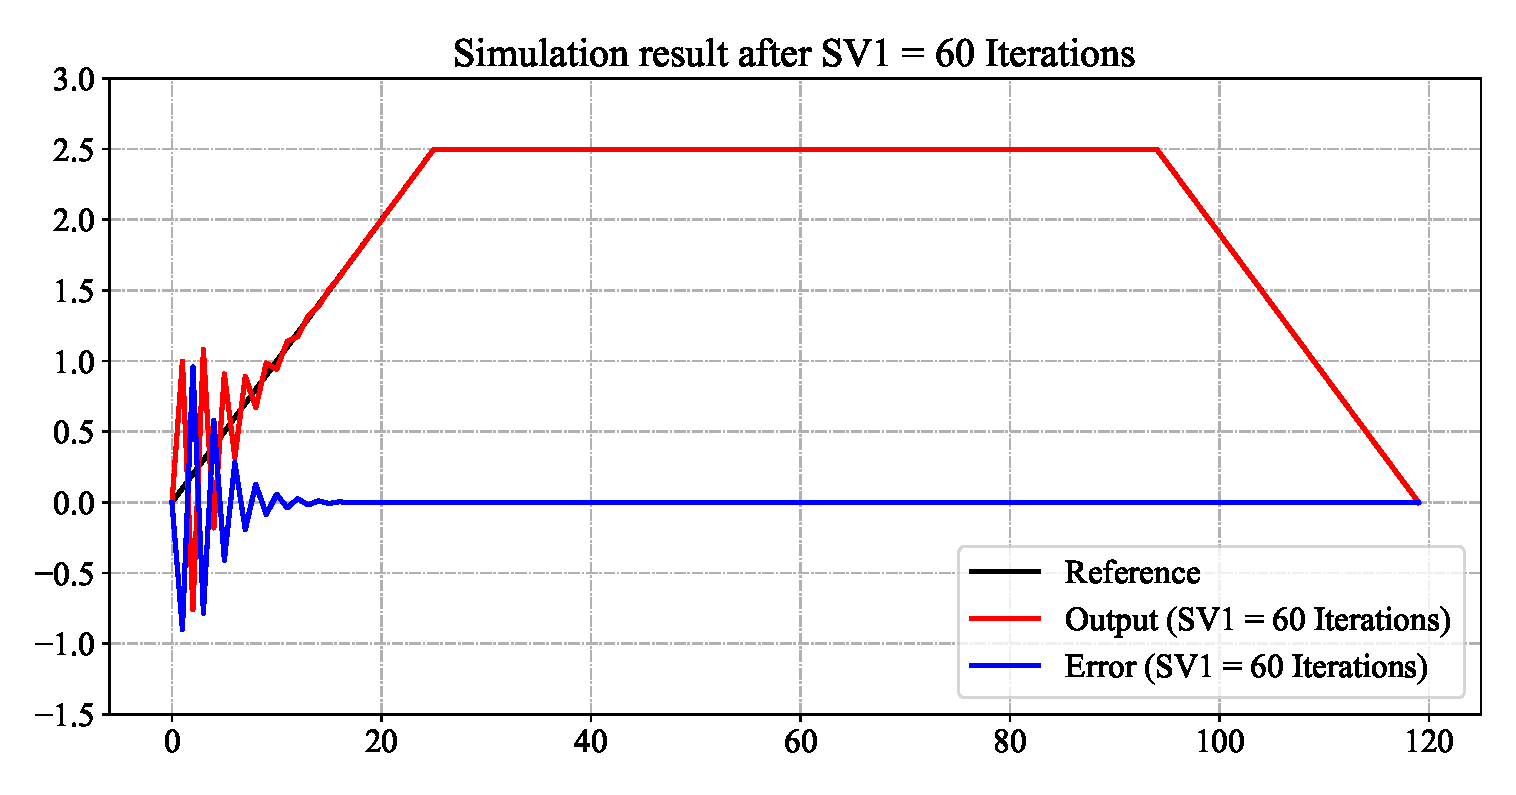
\includegraphics[width=\linewidth]{images/ICL_1.pdf}
	\caption{Simulation results at 60 iterations for the linear discrete-time plant in \eqref{eq:7}.}
	\label{fig:ICL_1}
\end{figure}

As shown in \autoref{fig:ICL_1}, the simulation results after 60 iterations demonstrate effective tracking performance. The reference and output exhibit close tracking, with minor deviations observed in the error plot, which remains bounded near zero. This indicates that the system has achieved a satisfactory level of convergence and tracking performance after 60 iterations.
\begin{figure}[ht]
	\centering
	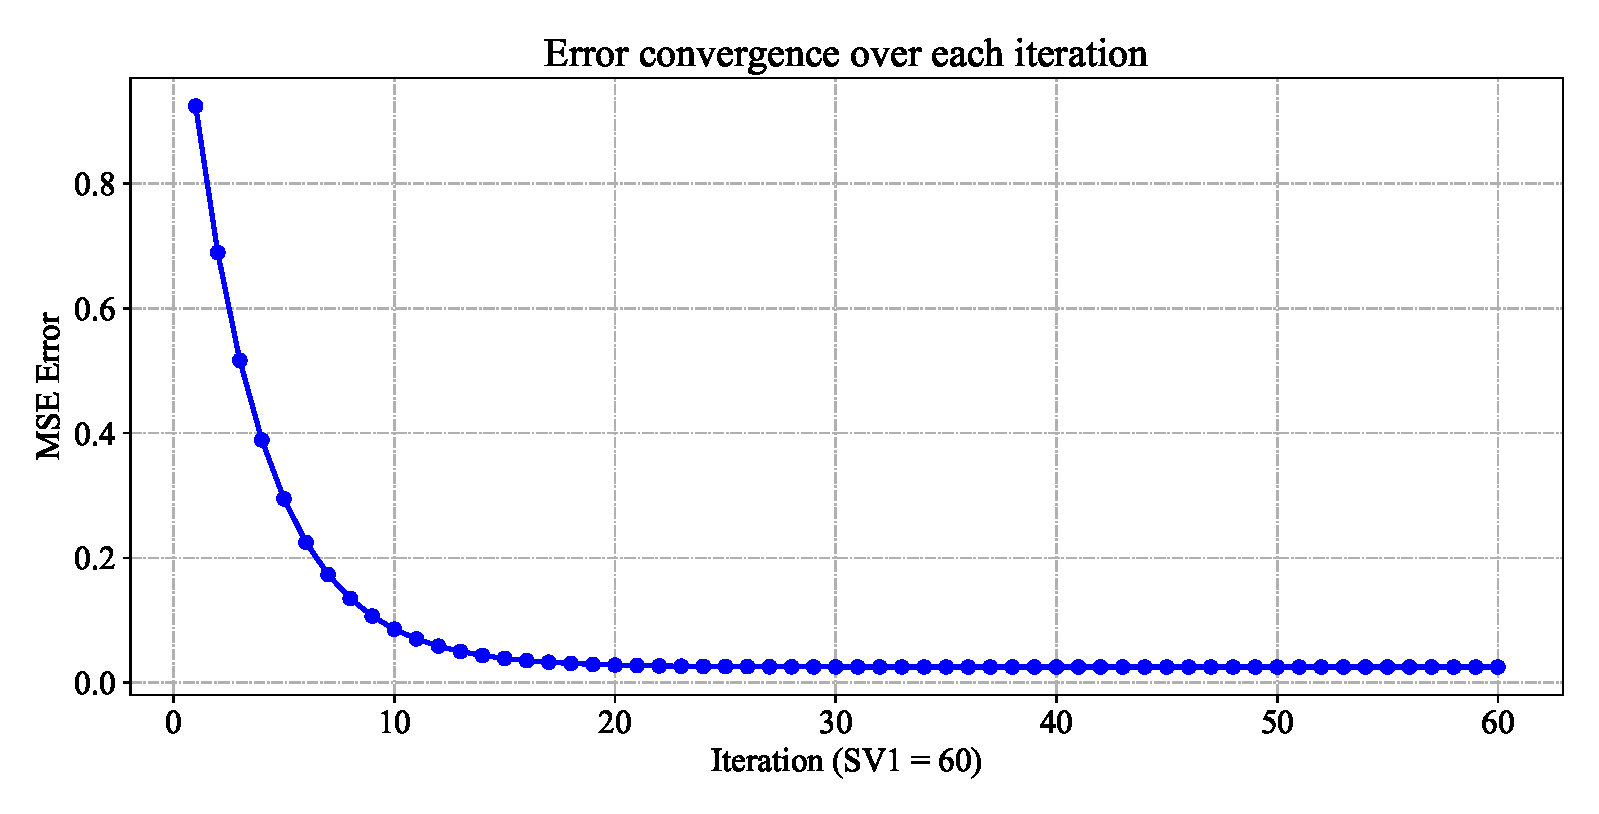
\includegraphics[width=\linewidth]{images/ICL_1_loss.pdf}
	\caption{Convergence of the Mean Squared Error (MSE) over iterations. The error decreases rapidly and stabilizes near zero after approximately 60 iterations.}
	\label{fig:ICL_1_loss}
\end{figure}
The convergence of the tracking error over iterations is illustrated in \autoref{fig:ICL_1_loss}. As the iteration count increases, the MSE decreases rapidly and converges to a small value near zero, demonstrating the effectiveness of the iterative learning control scheme for the linear discrete-time plant.
\subsection{Non-Linear discrete object}

Consider the nonlinear system described by the following state-space representation:
\begin{equation}
	\underline{\dot{x}} = \underline{f}(\underline{x}, u) = 
	\begin{pmatrix} 
		-x_1^3 + x_1 x_2 \\ 
		2x_1^2 - x_2 + u 
	\end{pmatrix}, \quad 
	y = g(\underline{x}) = x_2
\end{equation}
The system parameters and constraints are defined as:
\begin{itemize}
	\item Working Duration: $T = 140s$.
	\item Sampling Period: $T_s = 0.1s$.
	\item Initial Conditions: $\underline{x}_0 = \begin{pmatrix} 0 & 0.1 \end{pmatrix}^T$.
	\item Reference Trajectory: $r(t) = \sin\left(\frac{2\pi t}{T}\right)$.
\end{itemize}

\begin{figure}[ht]
	\centering
	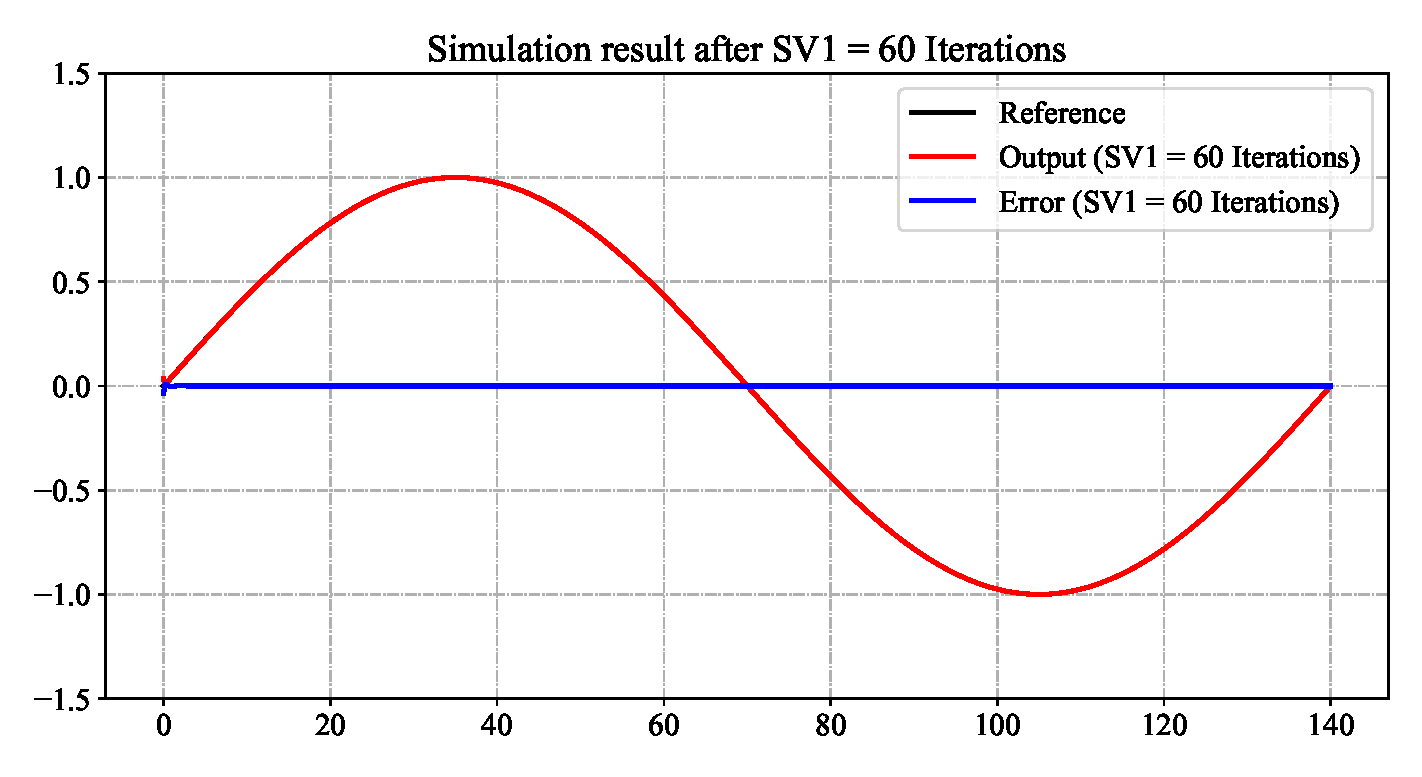
\includegraphics[width=\linewidth]{images/ICL_2.pdf}
	\caption{Simulation results for the nonlinear discrete-time plant at 60 iterations.}
	\label{fig:ICL_2}
\end{figure}

Given $T = 140$s and $T_s = 0.1s$, the total number of samples is:
\[
N = \frac{T}{T_s} = \frac{140}{0.1} = 1400.
\]
A PD-type iterative learning control law is selected as:
\begin{equation}
	u_{k+1}(\tau) = u_k(\tau) + K_1 e_k(\tau) + K_2 e_k(\tau + 1)
\end{equation}
where $k$ denotes the iteration index, $\tau \in [1, N]$ is the sample index, and $e$ represents the tracking error between $y(t)$ and $r(t)$. The controller gains are chosen as $K_1 = 0.1$ and $K_2 = 0.15$.
During each iteration and at each sampling step, the system state derivative is updated as:
\begin{equation}
	\dot{x} =
	\begin{bmatrix}
		\dot{x}_1 \\
		\dot{x}_2
	\end{bmatrix}
	=
	\begin{bmatrix}
		-x_1^3 + x_1 x_2 \\ 
		2x_1^2 - x_2 + u 
	\end{bmatrix}
\end{equation}
The output $y(t)$ at each sampling interval is obtained by integrating $\dot{x}_2$ over the sampling period $T_s$:
\begin{equation}
	y = \int_0^{T_s} \left( 2x_1^2 - x_2 + u  \right)\, dt
\end{equation}

The simulation results for the nonlinear discrete-time plant after 60 iterations are presented in \autoref{fig:ICL_2}. The tracking error remains bounded near zero, indicating successful convergence for the nonlinear discrete-time system.
\begin{figure}[ht]
	\centering
	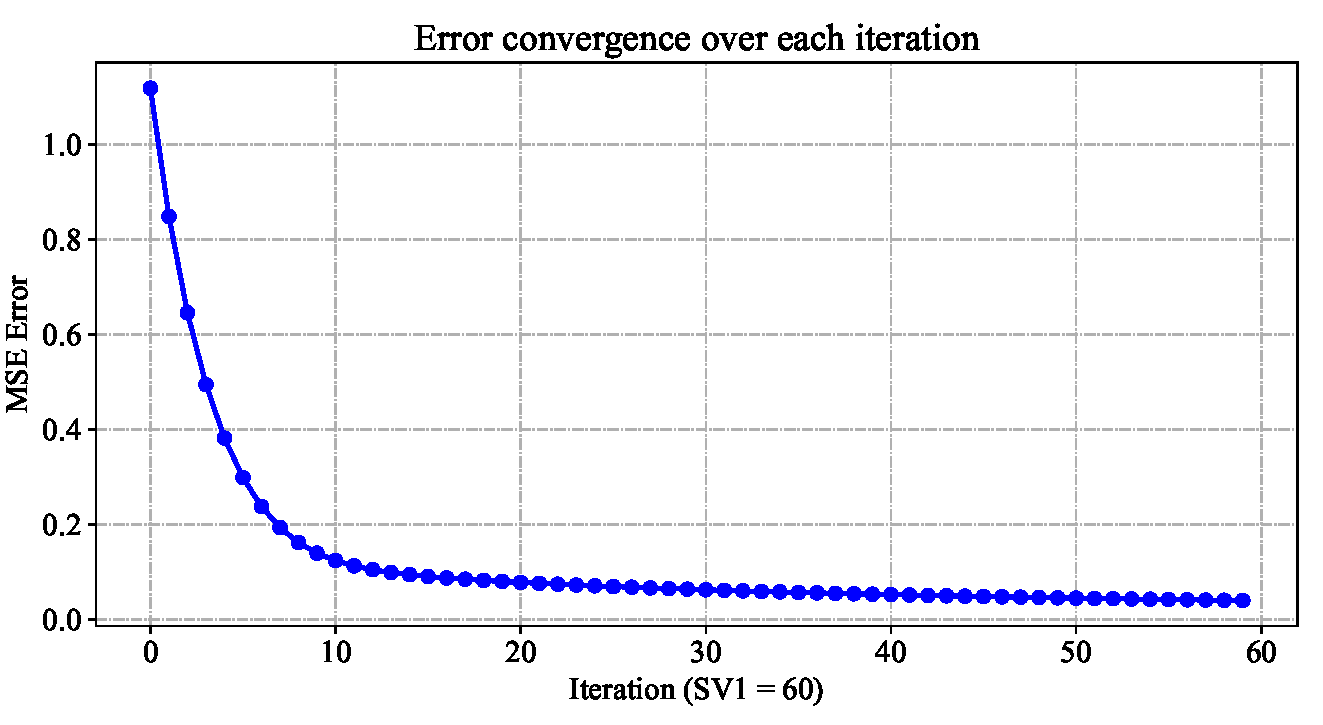
\includegraphics[width=\linewidth]{images/ICL_2_loss.pdf}
	\caption{MSE convergence over 60 iterations for the nonlinear discrete-time plant.}
	\label{fig:ICL_2_loss}
\end{figure}
The convergence of the tracking error over iterations for the nonlinear discrete-time plant is shown in \autoref{fig:ICL_2_loss}. As the iteration count increases, the MSE decreases rapidly and converges to a small value near zero, demonstrating the effectiveness of the iterative learning control scheme for the nonlinear discrete-time system.